\documentclass{article}
\usepackage[utf8]{inputenc}
\usepackage[spanish]{babel}
\usepackage{listings}
\usepackage{graphicx}
\graphicspath{ {./images/} }
\usepackage{cite}
\usepackage{wrapfig}

\begin{document}

\begin{titlepage}
    \begin{center}
        \vspace*{1cm}
            
        \Huge
        \textbf{Informe De Implementacion}
            
        \vspace{0.5cm}
        \LARGE
        Parcial 2
            
        \vspace{1.5cm}
            
        \textbf{Manuela Gutiérrez Rodríguez}
        \vspace{0.5cm}
        
        \textbf{Daniela Andrea Gallego Díaz}
            
        \vfill
            
        \vspace{0.8cm}
            
        \Large
        Despartamento de Ingeniería Electrónica y Telecomunicaciones\\
        Universidad de Antioquia\\
        Medellín\\
        21 de Septiembre de 2021
            
    \end{center}
\end{titlepage}

\tableofcontents
\newpage
\section{Clases implementadas}

Entre las clases que implementamos para la solucion de este problema fueron:

\subsection{Función submuestreo: }

\subsection{Funcion sobremuestreo:}
En esta funcion se implementan tres metodos, el constructor por defecto el cual tiene la funcion de recibir la ruta escrita por el usuario y almacenarla en un atributo privado de la clase para asi poder leer la imagen. Tambien un metodo llamdo lectura, que se encarga de leer cada pixel de la imagen de acuerdo al RGB y almacena cada valor en un vector de vectores (atributos privados de la clase), uno para los pixeles rojos, otro para los verdes y por ultimo los azules. El ultimo metodo implementado fue el de redimension, alli se hace el proceso de redimension de la imagen donde se itera sobre las matrices RGB y se van añadiendo pixeles teniendo encuenta las dimensiones originales y cuantos pixeles se deben agregar para llegar a una matriz de 12x12, en este mismo metodo almacenamos la matriz final ya redimensionada en un archivo .txt para asi utilizarlo como recurso para la implementacion en la plataforma de Tinkercard.


\section{Esquema de clases implementadas}
\subsection{Función submuestreo: }

\subsection{Funcion sobremuestreo:}
\begin{itemize}
\item Atributos privados de la clase:

\hspace{0.5cm}Variable string llamada ruta (almacena la ruta donde se encuentra la imagen seleccionada por el usuario)

\hspace{0.5cm}Un vector que contiene vectores, estos contienen las matrices segun el RGB (tres matrices en total por cada color)

\item Metodos de la clase:

\hspace{0.5cm}Sobremuestreo: Constructor por defecto, recibe un string el cual le da al atributo ruta la direccion que escribe el usuario, donde se encuentra la imagen a procesar.

\hspace{0.5cm}Lectura: Metodo que lee la imagen y almacena los valores de cada pixel en vectores que contienen vectores, cada uno segun el RGB.

\hspace{0.5cm}Redimension:Metodo que itera sobre cada una de las matrices RGB y va almacenando y agregando pixeles de acuerdo a las dimensiones de la imagen original para asi, en un archivo .txt tener todos los valores correspondientes con dimension 12x12.


\end{itemize}

\section{Modulos de codigo}

\section{Estructura del circuito}

Para la construcion del circuito hemos utilizado 12 tiras de 12 leds neopixel, para asi tener una dimension de 12x12.

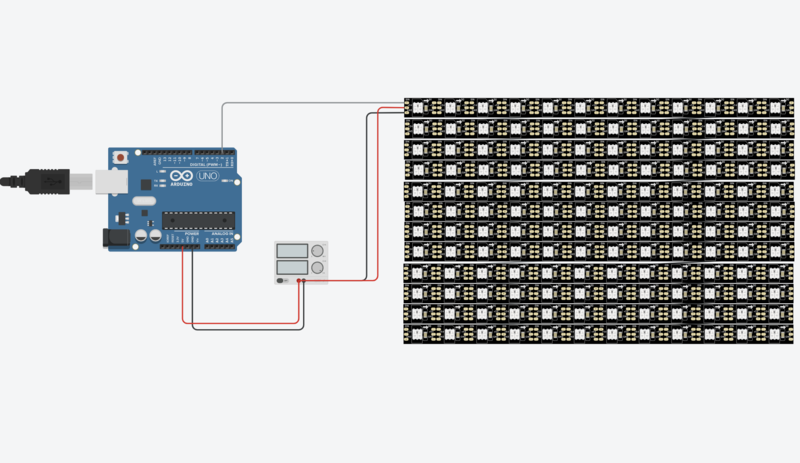
\includegraphics{images/Circuito.png}

\section{Problemas presentados}

\end{document}
